\documentclass{beamer}

%% Possible paper sizes: a0, a0b, a1, a2, a3, a4.
%% Possible orientations: portrait, landscape
%% Font sizes can be changed using the scale option.
\usepackage[size=a1,orientation=landscape,scale=1.4]
{beamerposter}
\usepackage{enumitem}
\usetheme{LLT-poster}
\setbeamertemplate{footline}
{
  \begin{beamercolorbox}[
    wd=\paperwidth,
    ht=1.5cm,        % ↓ hauteur du footer (clé)
    dp=0.5cm,
    center
  ]{author in head/foot}
    \usebeamerfont{author in head/foot}
    \insertshortauthor \hfill
    \insertshorttitle \hfill
    \insertshortinstitute
  \end{beamercolorbox}
}


\definecolor{accent}{RGB}{35,40,83}

\setbeamercolor{block title}{
  fg=white,
  bg=accent
}

\setbeamercolor{block body}{
  fg=black,
  bg=white
}

\setbeamercolor{normal text}{
  fg=black,
  bg=white
}

\setbeamercolor{headline}{
  fg=white,
  bg=accent
}

\setbeamercolor{title in headline}{
  fg=white
}

\setbeamercolor{author in headline}{
  fg=white
}

\setbeamercolor{institute in headline}{
  fg=white
}

\setbeamercolor{footline}{
  fg=white,
  bg=accent
}

\setbeamercolor{author in head/foot}{
  fg=white,
  bg=accent
}




% \usecolortheme{ConspiciousCreep}  %% VERY garish.
\usepackage{tikz}
\usetikzlibrary{positioning,fit,arrows.meta,calc}
\usepackage[utf8]{inputenc}
\usepackage[T1]{fontenc}
\usepackage{libertine}
\usepackage[scaled=0.92]{inconsolata}
\usepackage[libertine]{newtxmath}

\usepackage{mwe}
\definecolor{iclrblue}{RGB}{0,90,156}
\newcommand{\highlight}[1]{\textcolor{iclrblue}{\textbf{#1}}}


\author{Titouan Guerin \and  Yacine Chettab \and Louis Delsaer}
\title{GRLA: Bridging Softmax and Linear Attention via Gaussian RBF Kernel \\for lightweight image Super-Resolution}
\institute{Sorbonne Université}
\footimage{
\includegraphics[width=4cm]{Sorbonne-University.png}}
\begin{document}
\begin{frame}
\begin{columns}[T]


%%%% First Column
\begin{column}{.23\textwidth}
\begin{minipage}[t][\textheight][t]{\linewidth}

\begin{block}{Introduction}


La \textbf{super-résolution d’images} vise à reconstruire une image
haute résolution \textbf{HR} à partir d’une image basse résolution \textbf{LR}. Elle requiert la modé- lisation des dépendances spatiales pour restaurer les textures et les structures fines.

\par\vspace{0.5em}

\highlight{Défi.}
Les mécanismes d’attention à base de la fonction \textbf{Softmax} permettent de modéliser ces interactions globales,
au prix d’une complexité $o(n^2)$ peu adaptée aux modèles dits \textit{lightweight}.
\par\vspace{0.5em}

\highlight{Solution.}
Le papier introduit \textbf{MPB}, une architecture de super-résolution légère  reposant sur une \textbf{attention linéaire basée sur un noyau Gaussien (GRLA)}. Cette formulation conserve une \textbf{sensibilité à la distance} entre représentations, tout en maintenant une complexité linéaire.  



\end{block}





\begin{block}{Données}

\highlight{Entraînement.}
\par\vspace{0.2em}
\begin{itemize}
    \item \textbf{DIV2K} : 800 images en haute résolution (2K)
    \item Génération des images \textbf{LR} par \textbf{sous-échantillonnage bicubique} ($\times4$)
    \item Patches aléatoires $48 \times 48$ (LR)
    \item \textbf{Augmentation} : rotations, flips H/V
    \item Entraînement sur le \textbf{canal Y (YCbCr)}
\end{itemize}

\par\vspace{1em}

\highlight{Validation.}
\par\vspace{0.2em}
\begin{itemize}
    \item Benchmark avec des jeux de test: 
    \textbf{Set5}, \textbf{Set14} et \textbf{BSD100}
    \item Comparaison avec une \textbf{baseline bicubique}
    \item Suppression des {pixels de bord} pour éviter les artefacts d’upsampling
\end{itemize}

\par\vspace{1em}
Dépôt GitHub: \url{https://github.com/redscarfx/GRLA}.


\end{block}
\vfill
\hline
\vspace{0.4em}
\begin{description}[leftmargin=!]
\item[\highlight{RBF}] Radial Basis Function
\item[\highlight{GRLA/GRBFLA}] Gaussian RBF Linear Attention
\item[\highlight{SR}] Super-Resolved image
\item[\highlight{HR}] High-Resolution image
\item[\highlight{LR}] Low-Resolution image
\item[\highlight{PSNR}] Peak Signal-to-Noise Ratio
\item[\highlight{SSIM}] Structural Similarity Index Measure

\item[ ] 
\item[ ]
\end{description}

\end{minipage}





\end{column}

%%%% Second Column
\begin{column}{.48\textwidth}

\begin{block}{Méthode et modèle GRLA}

GRLA reformule l’attention Softmax comme un \textbf{noyau Gaussien RBF} \textbf{dépendant de la distance}:
\[
\begin{aligned}
K(Q_i, K_j)
&= \exp\!\left(-\gamma \|Q_i - K_j\|^2\right) 
&= \exp(-\gamma\|Q_i\|^2)\,
   \exp(-\gamma\|K_j\|^2)\,
   \exp(2\gamma Q_i^\top K_j).
\end{aligned}
\]



\vspace{1em}
À l’aide d’un \textbf{développement de Taylor d’ordre 1}: $
\exp(2\gamma Q_i^\top K_j) \approx 1 + 2\gamma Q_i^\top K_j.$
\vspace{1em}
\[
K(Q_i, K_j) \approx \phi(Q_i)\,\phi(K_j)\,(1 + 2\gamma Q_i^\top K_j) , \quad \phi(X) = \exp(-\gamma \|X\|^2).\]


\[
\alpha_i = 
\frac{
\sum_{j=1}^{N} \varphi(Q_i) \varphi(K_j)\bigl(1 + 2\gamma Q_i^\top K_j\bigr) V_j
}{
\sum_{j=1}^{N} \varphi(Q_i) \varphi(K_j)\bigl(1 + 2\gamma Q_i^\top K_j\bigr)
} =
\frac{
\sum_j \phi(K_j) V_j
\;+\;
2\gamma\, Q_i^\top \sum_j \phi(K_j) K_j V_j
}{
\sum_j \phi(K_j)
\;+\;
2\gamma\, Q_i^\top \sum_j \phi(K_j) K_j
} \sim {\mathcal{O}}(n)
\]
\begin{figure}
    \centering
    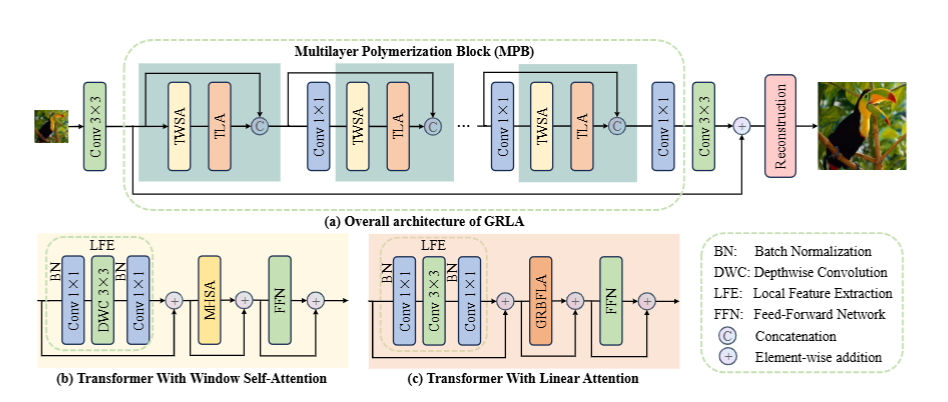
\includegraphics[width=1\linewidth]{arch.png}
    \caption{Architecture du modèle à base de GRLA de 7 blocs de $\langle TWSA + TLA \rangle $.}
    \label{fig:architecture}
\end{figure}


\vspace{0.4em}
Les performances sont évaluées à l’aide de métriques standards en super-résolution. Pour une vérité terrain $HR$ et une reconstruction $SR$ de la même résolution:

\[
\begin{aligned}
\mathrm{PSNR}(\mathrm{HR}, \mathrm{SR})
&= -10 \cdot \log_{10}\!\left(\frac{\mathrm{MSE}(\mathrm{HR}, \mathrm{SR})}{MAX^2}\right) \\[0.8em]
\mathrm{SSIM}(\mathrm{HR}, \mathrm{SR})
&=
\frac{\bigl(2\mu_{\mathrm{HR}} \mu_{\mathrm{SR}} + (k_1 L)^2\bigr)\bigl(2\sigma_{\mathrm{HR},\mathrm{SR}} + (k_2 L)^2\bigr)}
     {\bigl(\mu_{\mathrm{HR}}^2 + \mu_{\mathrm{SR}}^2 + (k_1 L)^2\bigr)\bigl(\sigma_{\mathrm{HR}}^2 + \sigma_{\mathrm{SR}}^2 + (k_2 L)^2\bigr)}  \qquad\text{avec } k_1 = 0.01,\quad k_2 = 0.03 .
\end{aligned}
\]


\vspace{1em}
\begin{itemize}
    \item \highlight{PSNR (dB) élevé} indique une \textbf{faible erreur pixel-à-pixel} entre les deux images $SR$ et $HR$. 
    Cette métrique, exprimée sur une \textbf{échelle logarithmique non bornée}, mesure principalement \textit{la ressemblance numérique}. $MAX$ est le pixel à valeur maximale dans les deux images. $MAX=1$ après la normalisation des données.
    \vspace{0.5em}
    
    \item \highlight{SSIM proche de 1} traduit une \textbf{forte similarité structurelle perceptuelle}. 
    Bornée dans $[0,1]$, cette métrique est mieux corrélée à la qualité visuelle ressentie en évaluant la cohérence des structures locales. $L$ représente la gamme dynamique. $L=1$ après la normalisation des données.
\end{itemize}

\end{block}







\end{column}

%%%% This is the THIRD column
\begin{column}{.23\textwidth}
\begin{block}{Résultats}
Le modèle de \textbf{MPB} avec 7 blocs a été entraîné pendant \textbf{170 epochs}
avec  \textbf{Adam} et une perte \textbf{L1 (MAE)}.


\begin{figure}
    \centering
    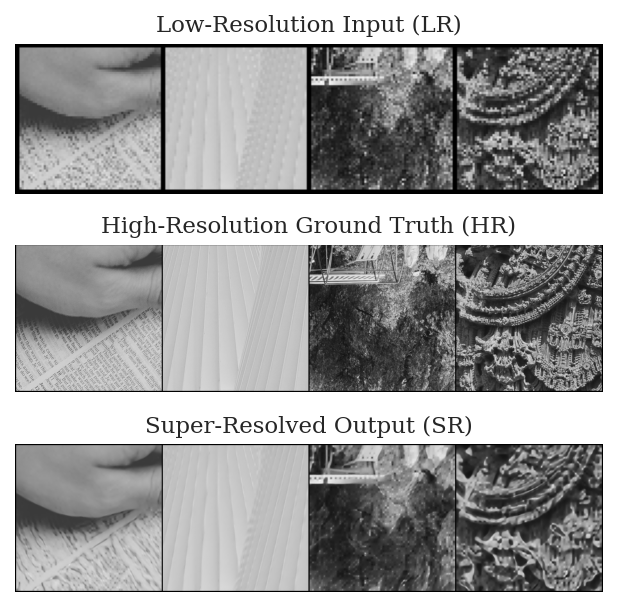
\includegraphics[width=0.9\linewidth]{batch.png}
    \caption{Exemples d’un batch avec 4 images en version LR, HR et SR prédite par le modèle.}
    \label{fig:batch_examples}
\end{figure}



\begin{table}[h]
\centering
\vspace{0.5em}
\begin{tabular}{lllll}
\toprule
\multicolumn{2}{c}{} & Bicubic& \multicolumn{2}{c}{\textbf{GRLA}} \\
 & & (baseline) & \textbf{(orig.)} & \textbf{(ours)} \\ 
\midrule
 & Params(K)  & --- & 885 & 863 \\ 
Set5 & PSNR (dB) & 27.66 & \textbf{32.64} & \underline{29.30} \\
     & SSIM (\%) & 81.32  & \textbf{90.01} & \underline{86.52} \\ 
\midrule
Set14 & PSNR (dB) & 24.54 & \textbf{28.89} & \underline{25.54} \\
      & SSIM (\%) & 68.99  & \textbf{78.80} & \underline{72.96}\\ 
\midrule
BSD100 & PSNR (dB) & 25.24 & \textbf{27.78} & \underline{25.93} \\
       & SSIM (\%) & 64.64  & \textbf{74.37} & \underline{66.20} \\
\bottomrule
\end{tabular}
\caption{Comparaison des performances en super-résolution $\times4$ entre l’interpolation bicubique, le modèle GRLA original et notre implémentation.
Le meilleur score est en \textbf{gras}, le second meilleur score est \underline{souligné}. La baseline Bicubic ne nécessite aucun paramètre à entraîner.}
\end{table}
\end{block}

\begin{block}{Conclusion}
L’entraînement limité à \textbf{170 epochs} (vs. 1000 dans le papier)
restreint la comparabilité des deux.
Le papier manque de détails sur les hyperparamètres, l’implémentation
et le prétraitement, ce qui limite la reproductibilité et l’évaluation des gains.
\end{block}





\end{column}


\end{columns}

\end{frame}
\end{document}